%TEX program = xelatex
\documentclass[12pt]{amsart}
\usepackage{tikz}
\usepackage{amssymb}
\usepackage{amsmath}
\usepackage{mathrsfs}
\usepackage{amsfonts}
\usepackage{amssymb,amsmath}
\usepackage{graphicx}
\graphicspath{{./images/}}
% \usepackage[pagewise]{lineno}\linenumbers
\oddsidemargin=-.0cm
\evensidemargin=-.0cm
\textwidth=16cm
\textheight=22cm
\topmargin=0cm
%%%%%%%%%%%%%%%%%%%%%%%%%%%%%%%%%%%%%%%%%%%%
% DEFS
\def\C {{\mathcal C}}

\def\R {\mathbb{R}}


\def\d{{\,\rm d}}

\def\i{{\rm i}}

%%%%%%%%%%%%%%%%%%%%%%%%%%%%%%%%%%%%%%%%%%%%

%%%%%%%%%%%%%%%%%%%%%%%%%%%%%%%%%%%%%%%%%%%%
\newtheorem{proposition}{Proposition}[section]
\newtheorem{theorem}[proposition]{Theorem}
\newtheorem{corollary}[proposition]{Corollary}
\newtheorem{lemma}[proposition]{Lemma}
\theoremstyle{definition}
\newtheorem{definition}[proposition]{Definition}
\newtheorem{example}[proposition]{Example}
\newtheorem{remark}[proposition]{Remark}
\numberwithin{equation}{section}
%%%%%%%%%%%%%%%%%%%%%%%%%%%%%%%%%%%%%%%%%%%%
% BIBLIOGRAPHY
\def \au {\rm}
\def \ti {\it}
\def \jou {\rm}
\def \bk {\it}
\def \no#1#2#3 {{\bf #1} (#3), #2.}
%\no{Vol}{Pag}{Year}
\def \eds#1#2#3 {#1, #2, #3.}
%\eds{Pub}{City}{Year}
%%%%%%%%%%%%%%%%%%%%%%%%%%%%%%%%%%%%%%%%%%%%%%%%%

\renewcommand\baselinestretch{1.3}

%%%%%%%%%%%%%%%%%%%%%%%%%%%%%%%%%%%%%%%%%%%%%%%%%
\title[Observability inequality ]
{ \bf
 Observability inequality at two time points for the KdV equation  from measurable sets}

%\author[ ]
%{Yunlei Wang }

\author[Y. Wang and M. Wang]
{Yunlei Wang and Ming Wang}

\address{Yunlei Wang and Ming Wang
\newline\indent
School of Mathematics and Physics, China University of Geosciences
\newline\indent
Wuhan, 430074, PR China
}
\email{mwang@cug.edu.cn}



\begin{document}
\begin{abstract}

We prove two observability inequalities at two time points for the linear KdV equation on the real line. In the two inequalities, the observable region in space is the complement of $(i)$ a measurable set with finite Lebesgue measure, and $(ii)$ of a measurable set contained in a half line with some density conditions, whose Lebesgue measure may be infinite.

\end{abstract}
%\keywords{KdV equation \and Global attractor \and Fractal dimension \and Bourgain space }
% \PACS{PACS code1 \and PACS code2 \and more}
%\subclass{35Q53  \and  35B41}

%\tableofcontents


\subjclass[2010]{35Q55, 39A12}
\keywords{KdV equation, observability,  unique continuation}
\maketitle
%%%%%%%%%%%%%%%%%%%%%%%%%%%%%%%%%%%%%%%%%%%%%%%%%



%%%%%%%%%%%%%%%%%%%%%%%%%%%%%%%%%%%%%%%%%%%%%%%%%





%%%%%%%%%%%%%%%%%%%%%%%%%%%%%%%%%%%%%%%%%%%%%%%%%
\section{Introduction}

The classical observability inequality for the Schr\"{o}dinger equation
\begin{align}\label{equ-sch}
i\partial_t u+\Delta u=0, \quad u(0,x)=u_0\in L^2(\R^n)
\end{align}
reads that when $u$ solves \eqref{equ-sch}
\begin{align}\label{sch-ob}
\int_{\R^n}|u_0(x)|^2\d x\leq C(n,T,E)\int_0^T\int_E|u(t,x)|^2\d x \d t,
\end{align}
where $T>0, E$ is a subset in $\R^n$ and $C(n,T,E)>0$ is a constant depending only on $n,T,E$. The inequality \eqref{sch-ob} holds if $E=\{x\in \R^n: |x|\geq r\}$ \cite{Rosier} in all dimensions $n\geq 1$, and $E$ is thick \cite{HWW} (a more general set class) in the dimension $n=1$. It is well known that the inequality \eqref{sch-ob} holds if and only if \eqref{equ-sch}, with controls restricted in $E$, is exactly controllable over $(0,T)$.

Recently,   Wang,  Wang and Zhang \cite{WWZ} have proved   the following new observability inequality: There exists a constant $C=C(n)>0$ such that for all $t>0$, all $r_1,r_2>0$ and all $u(t,x)$ solving \eqref{equ-sch},
\begin{equation}\label{sch-ob-1}
    \int_{\R^n}|u_0(x)|^2\d x \le C e^{\frac{Cr_1r_2}{t}}\left(\int_{|x|\ge r_1} |u_0(x)|^2\d x+\int _{|x|\ge r_2}|u(t,x)|^2\d x\right).
\end{equation}
This improves the inequality \eqref{sch-ob} since only two time points appear on the right hand side of \eqref{sch-ob-1}. By the same reason, \eqref{sch-ob-1} is called observability inequality at two time points. Moreover, it is also shown in \cite[Section 5.2]{WWZ} that the inequality \eqref{sch-ob-1} is equivalent to the exact controllability for the impulse controlled
free Schr\"{o}dinger equation at two time points, with controls restricted in the set outside of a ball at each time. Further observability inequalities at two time points are proved in \cite{Huang} for Schr\"{o}dinger equation with potentials and in \cite{wang21} for nonlinear Schr\"{o}dinger equations, respectively.

The proof of \eqref{sch-ob-1} is based on the uncertainty principle of Fourier transform, which roughly says that  it is impossible for a nonzero function and its Fourier transform to have compact supports simultaneously.
A quantitative version is the following inequality: There exists $C=C(n)>0$ so that for all $r_1,r_2>0$ and all $f\in L^2(\R^n)$
\begin{equation}\label{un}
    \int_{\R^n}|f(x)|^2\d x\le Ce^{Cr_1r_2}\left(\int_{|x|\ge r_1}|f|^2\d x+\int_{|x|\ge r_2}|\widehat{f}(\xi)|^2\d\xi\right),
\end{equation}
where $\widehat{f}$ denotes the Fourier transform of $f$, see e.g. \cite{Nazarov,Havin,Jaming}. Note that \cite{L-Ponce14} the solution of the Schr\"{o}dinger equation \eqref{equ-sch} satisfies the identity
\begin{align}\label{sch-relation}
(2it)^{\frac{n}{2}}e^{-i|x|^2/4t}u(x, t)=\widehat{e^{i|\cdot|^2/4t}u_0}(x/2t),\,\,\, \text{for all}\,\,t>0.
\end{align}
Roughly speaking, this means that the solution at time $t$ is the Fourier transform of the initial data $u_0$ up to a factor with modulus length $1$. With \eqref{sch-relation} in hand, the observability inequality \eqref{sch-ob-1} can be deduced from \eqref{un}. By the same way, it is also proved in \cite{WWZ} the following observability inequality. Let $A,B\subset \R^n$ be measurable sets with finite Lebesgue measure, namely $|A|,|B|<\infty$. Then for all $t>0$ and all solutions of \eqref{equ-sch}
\begin{equation}\label{sch-ob-2}
    \int_{\R^n}|u_0(x)|^2\d x \le C(t,A,B)\left(\int_{A^c} |u_0(x)|^2\d x+\int _{B^c}|u(t,x)|^2\d x\right),
\end{equation}
where $A^c$ denotes the complement set of $A$, $C(t,A,B)>0$ is a constant.

Since the Korteweg-de Vries (KdV) equation is also one of the most important dispersive equations, it is interesting to see whether the above observability inequality holds for  the linear  KdV  equation
\begin{equation}\label{kdv}
u_t+u_{xxx}=0, \quad u(0,x)=u_0(x)\in L^2(\R).
\end{equation}
But for the KdV equation \eqref{kdv}, no relation similar to \eqref{sch-relation} is available, thus the above argument proving \eqref{sch-ob-1} (or \eqref{sch-ob-2}) does not work now. Very recently,  Li and  Wang have proved in \cite{LW} the following analogue inequality of \eqref{sch-ob-1}: There exists a constant $C>0$ so that for all $r_1,r_2,t>0$ and all $u(t,x)\in C([0,\infty);L^2(\R))$ solving \eqref{kdv},
\begin{equation}\label{kdv-ob}
    \int_{\R}|u_0(x)|^2\d x\le Ce^{Ct^{-\frac{4}{3}}\left(r_1^4+r_2^4\right)}\left(\int_{|x|\ge r_1}|u_0(x)|^2\d x+\int _{|x|\ge r_2}|u(t,x)|^2\d x\right).
\end{equation}
The proof relies on a quantitative analytic smooth effect of the KdV equation with compact support data and a quantitative unique continuation inequality of analytic functions.

The main goal of this paper is to prove analogues of \eqref{sch-ob-2} for the KdV equation \eqref{kdv}. Our first result is as follows.
\begin{theorem}\label{thm-1}
    Let $A,B$ be two  measurable sets in $\R$ with finite measure. Then for every $t>0$, there exists $C=C(t,|A|,|B|)>0$ so that when $u(t,x)$ solves the KdV equation \eqref{kdv},
    \begin{equation}\label{kdv-ob-1}
    \int_\R |u_0|^2\d x \leq C\left( \int_{A^c}|u_0|^2\d x + \int_{B^c}|u(t,x)|^2\d x \right).
    \end{equation}
    \end{theorem}

Clearly, compared to the inequality \eqref{kdv-ob}, Theorem \ref{thm-1} is an improvement in the sense that it holds for more general sets $A$ and $B$. On the other hand, we note that the explicit dependence on $t,|A|,|B|$ of the constant $C$ is lost. The main reason is that our proof, different from that of \eqref{kdv-ob}, is based on a contradiction argument. The main idea is inspired by the proof of Amerin-Berthier uncertainty principle in \cite{Amrein}. The proof is split into three steps:
\begin{itemize}
  \item [(1)] Show that \eqref{kdv-ob-1} holds if
\begin{align}\label{equ-56-1}
  \|T\|_{L^2(\R)\to L^2(\R)}<1,
\end{align}
  where $T=\chi_BS(t)\chi_A$, $S(t)=e^{-t\partial_x^3}$ denotes the group generated by \eqref{kdv}.
  \item [(2)] Show that $T$ is a compact operator from $L^2(\R)$ to $L^2(\R)$.
  \item [(3)] One can reduce \eqref{equ-56-1} to $\|T\|_{L^2(\R)\to L^2(\R)}\neq 1$, which shall be proved by a contradiction argument using $(2)$.
\end{itemize}

In the proof of Theorem \ref{thm-1}, the assumption that $A$ and $B$ has finite measure is used in both step $(2)$ and step $(3)$. With a closer look at step $(2)$, we find that $T$ is still a compact operator if $A,B$ satisfy some density conditions, where $A,B$ may be sets with infinite measure. This will imply some new observability inequalities at two time points for the KdV equation. To state our result, we need the following definition.

%There is a major difference between  the result of Z. Li and M. Wang in \cite{LW} and Theorem \ref{thm-1}:
%The inequality (\ref{lw}) gives an exact relation between the constant and $t,r_1,r_2$. The inequality (\ref{kdv-obs}) fails to give such a relation, but removes the bounded condtion of two sets $A$ and $B$.
%
%
%Theorem \ref{thm-1} requires two sets $A$ and $B$ have finite measure. This limitation can be replaced by a more general condition (in which one of the sets may have infinite measure) in the case of Schr\"{o}dinger equations. We will find some type of  $A$ and $B$ with infinite measure and the inequality (\ref{kdv-obs}) still holds.

\begin{definition}
    We say the set $A\subset \R$ has $|x|^{-\alpha}$ density for some $\alpha>0$  if\footnote{Here and below, $A\lesssim B$ denote $A\leq CB$ for some not important constant $C>0$.}
    $$
    \varlimsup_{x\to \infty}|A\bigcap[x,x+1]|\cdot|x|^{\alpha}\lesssim 1.
    $$
\end{definition}
\begin{remark}\label{rem-1}
    It is equivalent to say that, there exists $L>0$ so that
    $$
        |A\bigcap[x,x+1]|\lesssim |x|^{-\alpha}, \quad \forall |x|\geq L.
    $$
\end{remark}


Our second result reads as follows.

\begin{theorem}\label{thm-2}
    Let  $A$ and $B$ be measurable sets with density $|x|^{-\alpha},$ $\alpha>\frac{5}{6}$. Assume further that either $A,B\subset (c,\infty)$ or $A,B\subset (-\infty,c)$  for some $c\in\R$. Then for every $t>0$, there exists $C=C(t,A,B)>0$ so that \eqref{kdv-ob-1} holds when $u(t,x)$  solves the KdV equation \eqref{kdv}.
\end{theorem}

In Theorem \ref{thm-2}, the most interesting case is $\alpha\in(\frac{5}{6},1]$, since if $\alpha>1$ then $A$ has finite Lebesgue measure, which has been treated in Theorem \ref{thm-1}. Let $\alpha\in (\frac{5}{6},1]$ and
$$
A=B=\bigcup_{k=1}^\infty [k,k+k^{-\alpha}].
$$
Then $A,B$ satisfy the assumptions of Theorem \ref{thm-2}, but have infinite Lebesgue measure. We assume in Theorem \ref{thm-2} that $A,B$ are contained in a half line for some technical reasons. We do not know whether the assumption can be removed.

Theorem \ref{thm-1} and Theorem \ref{thm-2} are quantitative version of the unique continuation property (UCP): If $u(0,\cdot)=0$ on $A^c$ and $u(t,\cdot)=0$ on $B^c$ with $t\neq 0$, then $u(t,x)\equiv 0$. Similar UCP results are proved by Zhang in \cite{zhang-kdv,zhang-sch}. Another kind of UCP, assuming $u(0,x)$ and $u(t,x)$ have some exponential decay on $x$, is established by Escauriaza,   Kenig, Ponce and Vega in \cite{EKPV-kdv} for KdV equations and in \cite{EKPV12} for Schr\"{o}dinger equations.

This paper is organized as follows. In Section 2, we give a general criterion for the observability at two time points of the KdV equation. In Section 3 and Section 4, we prove Theorem \ref{thm-1} and Theorem \ref{thm-2}, respectively.


\section{A general criterion}

In this section, we present a general criterion for the observability from two time points of the linear KdV equation. The main idea is inspired from the Hilbert space methods for the uncertainty principle of Fourier transform \cite[Part One, Chap. 3]{Havin}.

Let $S(t)=e^{-t\partial_x^3}$ be the solution group of linear KdV equation \eqref{kdv}. Then the solution of  \eqref{kdv} can be written as
\begin{align}\label{equ-kdv-solu}
u(t)=S(t)u_0=\int_\R G(t,x-y)u_0(y)\d y,
\end{align}
where $G$ is the fundamental solution of linear KdV equation, given by
\begin{align}\label{equ-kdv-ker}
    G(t,x)= \left\{
        \begin{array}{ll}
        \frac{1}{(3t)^{\frac{1}{3}}}\operatorname{Ai}(\frac{x}{(3t)^{\frac{1}{3}}}), & \hbox{ }t> 0 \\
        \delta(x), & \hbox{ }t=0.
        \end{array}
        \right.
\end{align}
Here, $\operatorname{Ai}(x)$ is the Airy function defined via
\begin{align*}
\operatorname{Ai}(x)= \frac{1}{2\pi}\int^{\infty}_{-\infty}e^{i(xz+\frac{1}{3}z^3)}\d z.
\end{align*}
According to \cite[p.330]{stein}, there exists a constant $C>0$ so that
\begin{align}\label{equ-Ai}
|\operatorname{Ai}(x)| \leq
\left\{
\begin{array}{ll}
C(1+|x|)^{-\frac{1}{4}}, &   x<0, \\
 Ce^{-\frac{2}{3}|x|^{\frac{3}{2}}}, &  x\geq 0.
\end{array}
\right.
\end{align}
We remark that \eqref{equ-kdv-ker}-\eqref{equ-Ai} will be used in Section 3-4. For the linear KdV equation \eqref{kdv}, the $L^2$ norm is conservative, namely
\begin{align}\label{equ-conservation-law}
\|S(t)u_0\|_{L^2(\R)}=\|u(t,\cdot)\|_{L^2(\R)}=\|u_0\|_{L^2(\R)}, \quad t\in \R.
\end{align}


Let $A,B$ be two measurable subsets of $\R$. Fix $t\in \R$. Define a linear operator $T:L^2(\R)\mapsto L^2(\R)$
\begin{align}\label{equ-T-def}
Tf = \chi_BS(t)\big( \chi_A f \big), \quad f\in L^2(\R).
\end{align}
Here and below, the characteristic function $\chi_A(x)=1$ if $x\in A$ and $\chi_A(x)=0$ if $x\notin A$. Thanks to the conservation law \eqref{equ-conservation-law}, it is easy to see that
\begin{align}\label{equ-T-norm}
\|T\|_{L^2(\R)\to L^2(\R)}\leq 1.
\end{align}



\begin{proposition}\label{prop-T}
Assume that $\|T\|_{L^2(\R)\to L^2(\R)}< 1$. Then there exists $C>0$ so that when $u(t,x)$ solves  \eqref{kdv}
$$
    \int_\R |u_0|^2\d x \leq C\left( \int_{A^c}|u_0|^2\d x + \int_{B^c}|u(t,x)|^2\d x \right).
$$
\end{proposition}
\begin{proof}
Assume that $\|T\|_{L^2(\R)\to L^2(\R)}=c_1$ for some $0\leq c_1<1$. Then, by definition \eqref{equ-T-def},
$$
\|\chi_B(x)S(t)(\chi_Au_0)\|_{L^2(\R)}\leq c_1\|u_0\|_{L^2(\R)}, \quad \forall u_0\in L^2(\R).
$$
This implies that
 $$
\|\chi_B(x)S(t) \chi_Au_0\|_{L^2(\R)}\leq c_1\|\chi_Au_0\|_{L^2(\R)}=c_1\|S(t) (\chi_Au_0)\|_{L^2(\R)}, \quad \forall u_0\in L^2(\R),
$$
where we used  $\|\chi_Au_0\|_{L^2(\R)}=\|S(t) (\chi_Au_0)\|_{L^2(\R)}$ (by \eqref{equ-conservation-law}) in the last step. From this, we deduce that
\begin{align*}
\|S(t) (\chi_Au_0)\|_{L^2(\R)}&\leq \|\chi_B(x)S(t) (\chi_Au_0)\|_{L^2(\R)}+\|\chi_{B^c}(x)S(t) (\chi_Au_0)\|_{L^2(\R)}\\
&\leq c_1\|S(t) (\chi_Au_0)\|_{L^2(\R)}+\|\chi_{B^c}(x)S(t) (\chi_Au_0)\|_{L^2(\R)},
\end{align*}
which implies that, with  $c_2=1/(1-c_1)$,
\begin{align}\label{equ-5}
 \|S(t) (\chi_Au_0)\|_{L^2(\R)}\leq c_2\|S(t) (\chi_Au_0)\|_{L^2(B^c)}, \quad \forall u_0\in L^2(\R).
\end{align}
Now we deduce from \eqref{equ-5} that
\begin{align*}
\|u_0\|_{L^2(\R)} &= \|S(t)u_0\|_{L^2(\R)}\leq \|S(t) (\chi_Au_0)\|_{L^2(\R)}+\|S(t) (\chi_{A^c}u_0)\|_{L^2(\R)}\\
&\leq c_2\|S(t) (\chi_Au_0)\|_{L^2(B^c)}+\|S(t) (\chi_{A^c}u_0)\|_{L^2(\R)}\\
&\leq c_2\|S(t)u_0\|_{L^2(B^c)}+(1+c_2)\|S(t) (\chi_{A^c}u_0)\|_{L^2(\R)}\\
&=c_2\|u(t,\cdot)\|_{L^2(B^c)}+(1+c_2)\|u_0\|_{L^2(A^c)}.
\end{align*}
This completes the proof.
\end{proof}

%\begin{remark}\label{rem-ST}

%\end{remark}




\section{Proof of Theorem \ref{thm-1}}

From Proposition \ref{prop-T}, the observability inequality from two time points follows from the bound $\|T\|_{L^2(\R)\to L^2(\R)}< 1$. For some technical reasons, we shall first show that
\begin{align}\label{equ-ST-0}
\|S(-t)T\|_{L^2(\R)\to L^2(\R)}<1,
\end{align}
and then using the fact
\begin{align}\label{equ-ST}
\|T\|_{L^2(\R)\to L^2(\R)}=\|S(-t)T\|_{L^2(\R)\to L^2(\R)},
\end{align}
to conclude that $\|T\|_{L^2(\R)\to L^2(\R)}< 1$. We remark that \eqref{equ-ST} is a direct consequence of  the conservation law \eqref{equ-conservation-law}. The main part of this section is to prove \eqref{equ-ST-0} for some sets $A$ and $B$.

We adopt the strategy of Amerin and Berthier in \cite{Amrein}. Thanks to Proposition \ref{prop-T} and \eqref{equ-ST}, Theorem  \ref{thm-1} follows from the following proposition.
\begin{proposition}\label{prop-3}
Let $A$, $B$ be two measurable sets in $\R$ with finite Lebesgue measure, namely $|A|,|B|<\infty$. Let $S(t)$ and $T$ be given by \eqref{equ-kdv-solu} and \eqref{equ-T-def}, respectively. Then for all $t>0 0$ we have
$$
\|S(-t)T\|_{L^2(\R)\to L^2(\R)}<1.
$$
\end{proposition}

To prove Proposition \ref{prop-3}, we need some lemmas.

\begin{lemma}\label{lem-T-comp}
For every $t>0$, $T$ is a compact operator from $L^2(\R^n)$ to $L^2(\R^n)$.
\end{lemma}
\begin{proof}
By \eqref{equ-kdv-solu} and \eqref{equ-T-def}, we can rewrite the operator $T$ as an integral operator:
$$
(Tf)(x)=\int_{\R }\chi_A(x)G(t,x-y)\chi_B(y)f(y)\d y:=\int_{\R } K(t,x,y)f(y)\d y.
$$
We claim that for all $t>0$,
\begin{align}\label{equ-10}
 \int_{\R }\int_{\R } K^2(t,x,y)\d x \d y<\infty.
\end{align}
Then $T$ is a Hilbert-Schmidt operator and thus a compact operator on $L^2(\R )$, see e.g. \cite[p.277]{Yosida}.

It remains to show \eqref{equ-10}. In fact, for every $t>0$, we deduce from \eqref{equ-kdv-ker} and \eqref{equ-Ai} that $|G(t,x-y)|\leq C(t)$, where $C(t)>0$ is a constant depending only on $t$. Then
\begin{align*}
 \int_\R\int_\R K^2(t,x,y)\d x \d y\leq  C^2(t) \int_\R\int_\R \chi_A(x)\chi_B(y)d x \d y=C^2(t)|A||B|<\infty.
\end{align*}
This proves \eqref{equ-10}.
\end{proof}

Let $f$ be a measurable function on $\R$ and $A$ be a measurable set. We say that the support $\mathrm{supp } \, f\subset A$ if
$$
f(x)=0, \quad a.e. \, x\in A^c.
$$

\begin{lemma}\label{lem-2}
Suppose that $\|\chi_BS(t)(\chi_Af)\|_{L^2(\R)}=\|f\|_{L^2(\R)}$ for some $f\in L^2(\R)$, then the support $\mathrm{supp } \, f\subset A$
and $\mathrm{supp } \, S(t)f \subset B$.
\end{lemma}
\begin{proof}
We first show that
\begin{align}\label{equ-425-1}
\mathrm{supp }  \, f\subset A.
\end{align}
We argue by contradiction. Suppose that
$$
\Big|\{x\in \R: |f(x)|>0\} \backslash A \Big|>0.
$$
This implies that
\begin{align}\label{equ-425-2}
\|f\|_{L^2(A^c)}>0.
\end{align}
But by the assumption
$$
\|f\|_{L^2(\R)}=\|\chi_BS(t)(\chi_Af)\|_{L^2(\R)}\leq \|\chi_Af\|_{L^2(\R)},
$$
which implies that $\|f\|_{L^2(A^c)}=0$. This leads a contradiction with \eqref{equ-425-2}. So \eqref{equ-425-1} holds.

Using \eqref{equ-425-1} and the assumption, we deduce that
$$
\|\chi_BS(t)f\|_{L^2(\R)}=\|\chi_BS(t)(\chi_Af)\|_{L^2(\R)}=\|f\|_{L^2(\R)}=\|S(t)f\|_{L^2(\R)}.
$$
This gives that $\mathrm{supp } \, S(t)f \subset B$.
\end{proof}

For $\lambda\in \R$ and $A\subset\mathbb{R}$, we denote by $A+\lambda=\{x\in \mathbb{R}\lvert x+\lambda \in A\}$.
\begin{lemma}\label{lem-3}
Let $C_0\subset C$ be two measurable sets in $\R$ satisfying $0<|C_0|,|C|<\infty$. Define a function
$$
h_C(\lambda)=|C\cup (C_0+\lambda)|, \quad \lambda\geq 0.
$$
Then $h_C$ is a continuous function of $\lambda$, $h(0)=|C|$ and $\lim_{\lambda\to \infty}\limits h_C(\lambda)=|C|+|C_0|$.
\end{lemma}
\begin{proof}
See \cite[p.99]{Havin}.
\end{proof}

We need the following lemma, which is a variant version of \cite[Lemma 1]{Amrein}.

\begin{lemma}\label{lem-4}
Let $C_0\subset C, D_0\subset D$ be four measurable sets in $\mathbb{R}$ satisfying $0<|C_0|, |C|$, $|D_0|, |D|<\infty$. Then for every $\varepsilon>0$, there  exists a translation $\lambda>0$ such that
\begin{align}\label{equ-426-1}
   |C\cup (C_0+\lambda)|\leq|C|+\varepsilon, \quad    |D\cup (D_0+\lambda)|\leq|D|+\varepsilon
\end{align}
and either
\begin{align}\label{equ-426-2}
  |C|<|C\cup (C_0+\lambda)|
\end{align}
or
\begin{align}\label{equ-426-3}
 |D|< |D\cup (D_0+\lambda)|.
\end{align}
\end{lemma}
\begin{proof}
Define two functions
$$
h_C=|C\cup (C_0+\lambda)|, \quad h_D=|D\cup (D_0+\lambda)|, \quad \lambda\geq 0.
$$
Fix $\varepsilon>0$. Consider the level set
$$
\{h_C=|C|+\varepsilon\}=\{\lambda\geq 0: h_C(\lambda)=|C|+\varepsilon\}.
$$
Thanks to Lemma \ref{lem-3}, $h_C$ is a continuous function of $\lambda$, $h(0)=|C|$ and $\lim_{\lambda\to \infty}\limits h_C(\lambda)=|C|+|C_0|$. Thus $\{h_C=|C|+\varepsilon\}$ is a nonempty closed set. Put
$$
\lambda'=\min_{\lambda\in h_C=|C|+\varepsilon} \lambda.
$$
Then by the continuity of $h_C$ again, we have
\begin{align}\label{equ-426-4}
|C|\leq h_C(\lambda)\leq|C|+\varepsilon, \quad \forall \lambda\in[0,\lambda'].
\end{align}
We divide the discussion into two cases.

{\bf Case 1:} $h_D(\lambda')\leq |D|+\varepsilon$. This, together with the fact $h_C(\lambda')=|C|+\varepsilon$, implies that \eqref{equ-426-1} and \eqref{equ-426-2} hold with $\lambda=\lambda'$.

{\bf Case 2:} $h_D(\lambda')>|D|+\varepsilon$. Applying Lemma \ref{lem-3} to $h_D$, we find that
$$
 h_D(\lambda'')=|D|+\varepsilon
$$
for some $\lambda''\in(0,\lambda')$. Moreover, by \eqref{equ-426-4} we have
$$
|C|\leq h_C(\lambda'')\leq|C|+\varepsilon.
$$
Thus, in this case, \eqref{equ-426-1} and \eqref{equ-426-3} hold with $\lambda=\lambda''$.
\end{proof}



\begin{proof}[\bf \textit{Proof of Proposition \ref{prop-3}}.] %If either $|A|=0$ or $|B|=0$, the conclusion holds clearly. Thus we assume from now on that
%\begin{align}\label{equ-426-0}
%|A|,|B|>0.
%\end{align}
First of all, by \eqref{equ-conservation-law} and \eqref{equ-T-norm}, we have the trivial bound
$$
\|S(-t)T\|_{L^2(\R)\to L^2(\R)}\leq 1.
$$
Thus Proposition \ref{prop-3} holds if one can show that, for all $t>0$
\begin{align}\label{equ-4-23-1}
\|S(-t)T\|_{L^2(\R)\to L^2(\R)}\neq 1.
\end{align}


To show this, we use the contradiction argument. Fix $t>0$. Suppose that
\begin{equation}\label{assum}
    \|S(-t) T \|_{L^2(\R)\to L^2(\R)}=1.
\end{equation}
Since $\|S(-t)\|_{L^2(\R)\to L^2(\R)}=1$ and, by Lemma \ref{lem-T-comp}, $T$ is a compact operator on $L^2(\R)$, we find that $S(-t)T$ is a compact operator on  $L^2(\R)$. This, together with \eqref{assum}, implies that there exists a function $f\in L^2(\R)$ such that
\begin{align}\label{equ-425-3}
\|S(-t)Tf\|_{L^2(\R)}=\|f\|_{L^2(\R)}=1.
\end{align}
Since $\|S(-t)Tf\|_{L^2(\R)}=\|Tf\|_{L^2(\R)}$, by \eqref{equ-425-3}, we have $\|Tf\|_{L^2(\R)}=\|f\|_{L^2(\R)}$. Then, by Lemma \ref{lem-2}, we find
\begin{align}\label{equ-425-4}
\mathrm{supp } f\subset A, \quad \mathrm{supp }\,  S(t)f\subset B.
\end{align}
Set
$$
A_0=\mathrm{supp } f, \quad B_0=\mathrm{supp }\,  S(t)f.
$$
By the assumption on $A,B$ and \eqref{equ-425-4} we know that
\begin{align}\label{equ-425-10}
0<|A_0|, |B_0|<\infty.
\end{align}
Thanks to \eqref{equ-425-10}, we can apply Lemma \ref{lem-3} to find a sequence $\{\lambda_i\}_{i=1}^\infty\subset(0,\infty)$ such that
\begin{align}\label{equ-425-5}
|A_{i-1}\cup (A_0+\lambda_i)|\leq |A_{i-1}|+\frac{1}{2^i}, \quad   |B_{i-1}\cup (B_0+\lambda_i)|<|B_{i-1}|+\frac{1}{2^i}
\end{align}
and
\begin{align}\label{equ-425-6}
\mbox{either } |A_{i-1}|< |A_{i-1}\cup (A_0+\lambda_i)|  \quad  \mbox{ or } \quad |B_{i-1}|< |B_{i-1}\cup (B_0+\lambda_i)|,
\end{align}
where for $i=1,2,\cdots,$
\begin{align}\label{equ-425-7}
A_i=A_{i-1}\cup  (A_0+\lambda_i), \quad B_i=B_{i-1}\cup (B_0+\lambda_i).
\end{align}
It follows from \eqref{equ-425-5}-\eqref{equ-425-7} that
\begin{align}\label{equ-425-8}
|\bigcup_{i=0}^{\infty}A_i|\leq |A|+1,\quad |\bigcup_{i=0}^{\infty}B_i|\leq|B|+1.
\end{align}
Define $f_0=f$ and
$$
f_i=\mathcal{T}_{\lambda_i}f, \quad i=1,2,\cdots.
$$
where $\mathcal{T}_\lambda$ is the translation operator, namely
\begin{equation*}
    \mathcal{T}_{\lambda}f(x)=f(x-\lambda).
\end{equation*}
It is easy to see that   $\mathrm{supp}\, f_\lambda=A_0+\lambda$ and $S(t)f_\lambda=\mathcal{T}_{\lambda}(S(t)f)$, thus  $\mathrm{supp}\,S(t)f_\lambda= B_0+\lambda$. Then for $i=1,2,\cdots$
\begin{align}\label{equ-426-5}
\mathrm{supp }f_i=A_0+\lambda_i\subset A_i, \quad \mathrm{supp}\,S(t)f_i =B_0+\lambda_i\subset B_i.
\end{align}
Let $\mathcal {A}=\bigcup_{i=0}^{\infty}A_i$ and $\mathcal {B}=\bigcup_{i=0}^{\infty}B_i$. We have the following claims.
\begin{itemize}
  \item [(i)] The sequence $\{ f_i\}_{i=0}^{\infty}$ are linearly independent.
  \item [(ii)]  The operator $S(-t)\chi_\mathcal {B}S(t)\chi_\mathcal {A}$ is compact on $L^2(\R)$.
  \item [(iii)]  For all $i=0,1,\cdots,$ $f_i$ are the eigenfunctions of $S(-t)\chi_\mathcal {B}S(t)\chi_\mathcal {A}$ corresponding to the eigenvalue $1$.
\end{itemize}

To show $(i)$, we fix $m\in \mathbb{N}$. Thanks to \eqref{equ-425-6} and \eqref{equ-426-5}, we have either $\chi_{A_m\setminus A_{m-1}}f_m\neq 0$ or $\chi_{B_m\setminus B_{m-1}}S(t)f_m\neq 0$. In both cases it can be shown that $f_m$ is not a linear combination of $f_0,f_1,\cdots,f_{m-1}$. This means that the sequence $\{f_i\}_{i=0}^{m}$ are linearly independent. Thus $(i)$ holds.

For $(ii)$, we first note that $|\mathcal {A}|,|\mathcal {B}|<\infty$ since \eqref{equ-425-8}. Then by Lemma \ref{lem-T-comp}, we find that $S(-t)\chi_\mathcal {B}S(t)\chi_\mathcal {A}$ is compact.

For $(iii)$,  by \eqref{equ-426-5} and the definition of $\mathcal {A}$ and $\mathcal {B}$, we have
$$
\mathrm{supp } f_i\subset \mathcal {A}, \quad \mathrm{supp }\,  S(t)f_i\subset \mathcal {B}
$$
for all $i=0,1,\cdots$. Hence
$$
S(-t)Tf_i=S(-t)\chi_{\mathcal {B}}S(t)(\chi_{\mathcal {A}}f_i)=S(-t)\chi_{\mathcal {B}}S(t)f_i=S(-t)S(t)f_i=f_i.
$$
Namely, for every $i$, $f_i$ is an eigenfunction of $S(-t)\chi_\mathcal {B}S(t)\chi_\mathcal {A}$ corresponding to the eigenvalue $1$. Thus $(iii)$ holds.

Finally, the claims $(i)$ and $(iii)$ imply that   the  operator $S(-t)\chi_\mathcal {B}S(t)\chi_\mathcal {A}$  has infinitely many linearly independent eigenfunctions corresponding to the eigenvalue $1$, which contradicts to the compact property in $(ii)$. This shows that the assumption  (\ref{assum}) is invalid. Thus \eqref{equ-4-23-1} holds.
\end{proof}

\section{Proof of Theorem \ref{thm-2}}

We shall prove a more general theorem than Theorem \ref{thm-2} in this section. In fact, if $\alpha=\beta>\frac{5}{6}$, then $(\alpha,\beta)$ satisfy that
$$
  ({\bf H}) \qquad   \qquad \qquad   \begin{cases}
          \alpha+\beta>\frac{5}{3}&\\
          \alpha+3\beta>3&\\
          3\alpha+\beta>3&\\
          \alpha,\beta>\frac{1}{2}&
       \end{cases}.
        \qquad \qquad \qquad
$$
Thus, Theorem \ref{thm-2} is a direct consequence of the follow theorem.

\begin{theorem}\label{thm-4}
Let $(\alpha,\beta)$ satisfy the condition $({\bf H})$. Assume that  $A$ and $B$ are measurable sets with density  $|x|^{-\alpha}$ and $|x|^{-\beta}$, respectively. Assume further that either  $A,B\subset (c,\infty)$ or $A,B\subset (-\infty,c)$  for some constant $c\in \R$. Then for every $t>0$, there exists $C=C(t,A,B)>0$ so that when $u(t,x)$  solves the KdV equation \eqref{kdv},
$$
    \int_\R |u_0|^2\d x \leq C\left( \int_{A^c}|u_0|^2\d x + \int_{B^c}|u(t,x)|^2\d x \right).
$$
\end{theorem}

The idea is still to use Proposition \ref{prop-T}, namely to show $\|T\|_{L^2(\R)\to L^2(\R)}<1$, where
\begin{align}\label{equ-51-1}
Tf=\chi_BS(t)\chi_A f = \int_\R K(t,x,y)f(y)\d y, \quad f\in L^2(\R)
\end{align}
and
\begin{align}\label{equ-51-2}
K(t,x,y)=\chi_B(x)G(t,x-y)\chi_A(y)f(y).
\end{align}
Here $S(t)=e^{-t\partial_x^3}$ and $G$ is given by \eqref{equ-kdv-ker}.


\begin{lemma}\label{lem-comp-2}
Let $(\alpha,\beta)$ satisfy the condition $({\bf H})$. Assume that  $A$ and $B$ are measurable sets with density $|x|^{-\alpha}$ and $|x|^{-\beta}$, respectively. Then the kernel $K$, given by \eqref{equ-51-2}, satisfies
    $$
       \int_{\mathbb{R}}\int_{\mathbb{R}}K^2(t,x,y)\d x\d y<\infty.
    $$
 \end{lemma}

 \begin{proof}
Thanks to \eqref{equ-51-2}, \eqref{equ-kdv-ker} and \eqref{equ-Ai}, it suffices to show that
    \begin{equation}
       \int_{\mathbb{R}}\int_{\mathbb{R}}\chi_B(x)\langle|x-y|\rangle^{-\frac{1}{2}}\chi_A(y)\d x\d y<\infty.\label{eqn1-1}
    \end{equation}
Here and below, $\langle x \rangle = 1+|x|$.
    Rewrite the left hand side of \eqref{eqn1-1}  as
    \begin{equation}
       \sum_{j\in \mathbb{Z}}\sum_{k\in\mathbb{Z}}\int_j^{j+1}\int_k^{k+1}\chi_B(x)\langle|x-y|\rangle^{-\frac{1}{2}}\chi_A(y)\d x\d y.\label{eqn1-2}
    \end{equation}
    But when $x\in [k,k+1]$, $y\in[j,j+1]$, then
    $$
       \langle|x-y|\rangle\sim \langle|j-k|\rangle.
    $$
Here $A\sim B$ means that both $A\lesssim B$ and $B\lesssim A$ hold.
    Now (\ref{eqn1-2}) is bounded by
    \begin{align}
       &\sum_{j\in \mathbb{Z}}\sum_{k\in\mathbb{Z}}\int_j^{j+1}\int_k^{k+1}\chi_B(x)\langle|j-k|\rangle^{-\frac{1}{2}}\chi_A(y)\d x\d y\notag\\
       =&\sum_{j\in\mathbb{Z}}\sum_{k\in\mathbb{Z}}|B\cap [k,k+1]|\cdot \langle|j-k|\rangle^{-\frac{1}{2}}\cdot |A\cap [j,j+1]|\notag\\
       \lesssim & 1+\sum_{j,k\in\mathbb{Z},|j|,|k|\ge L} |B\cap[k,k+1]|\cdot \langle|j-k|\rangle^{-\frac{1}{2}}\cdot|A\cap [j,j+1]|\notag\\
       \lesssim & \sum_{j,k\in\mathbb{Z},|j|,|k|\ge L} |j|^{-\alpha}|k|^{-\beta}\langle |j-k|\rangle^{-\frac{1}{2}}.\label{eqn1-3}
    \end{align}
In the last line of \eqref{eqn1-3}, we have used Remark \ref{rem-1}.
 Split the sum in \eqref{eqn1-3} as
 \begin{align}\label{equ-426-10}
 \sum_{j,k\in\mathbb{Z},|j|,|k|\ge L} |j|^{-\alpha}|k|^{-\beta}\langle |j-k|\rangle^{-\frac{1}{2}}:= I+II,
 \end{align}
 where $I, II$ taking sum over  $|j|\leq |k|$ and $|j|>|k|$, respectively.

{\bf Estimate of $I$.} Let $\delta\in (0,1)$ to be determined later. Make further decomposition
$I:=I_1+I_2$,  where
 \begin{align}
I_1 &= \sum_{|j|,|k|\ge L, |k|-|k|^\delta\leq |j|\leq |k|} |j|^{-\alpha}|k|^{-\beta}\langle |j-k|\rangle^{-\frac{1}{2}},\label{equ-426-14}\\
I_2 &= \sum_{|j|,|k|\ge L, |j|> |k|-|k|^\delta} |j|^{-\alpha}|k|^{-\beta}\langle |j-k|\rangle^{-\frac{1}{2}}.\label{equ-426-15}
 \end{align}
For $I_1$,  since $|k|-|k|^\delta\le |j|\le |k|$, we have
\begin{align}\label{equ-426-16}
       I_1       \le  \sum_{|k|\ge L,|k|-|k|^\delta\le|j|\le |k|}|j|^{-\alpha}|k|^{-\beta}
       \lesssim  \sum_{|k|\ge L}|k|^{\delta-\alpha}|k|^{-\beta}=\sum_{|k|\ge L}|k|^{\delta-\alpha-\beta}.
\end{align}
For $I_2$, since $|j|<|k|-|k|^\delta$, we have $|k-j|\ge |k|-|j|\ge |k|^\delta$, then  $\langle |j-k| \rangle^{-1}\lesssim|k|^{-\delta}$. We split the discussion into two cases.
     \begin{itemize}
        \item  $0<\alpha\leq 1$, we have
     \begin{align}
        I_2&= \sum_{|k|\ge L,|j|<|k|-|k|^\delta}|j|^{-\alpha}|k|^{-\beta}\langle |j-k|\rangle^{-\frac{1}{2}}\lesssim \sum_{|k|\ge L,|j|<|k|-|k|^{\delta}}|j|^{-\alpha}|k|^{-\beta-\frac{1}{2}\delta}\nonumber\\
        &\lesssim
     \left\{
     \begin{array}{ll}
     \sum_{|k|\ge L }\limits|k|^{1-\alpha}|k|^{-\beta-\frac{1}{2}\delta}=\sum_{|k|\ge L}\limits|k|^{1-\frac{1}{2}\delta-\alpha-\beta}, \quad & 0<\alpha<1, \vspace{1ex}\\
      \sum_{|k|\ge L }\limits\ln|k|\cdot|k|^{-\beta-\frac{1}{2}\delta}, \quad & \alpha=1.
     \end{array}
     \right. \label{equ-426-17}
     \end{align}

       \item $\alpha>1$, we have
    \begin{align}\label{equ-426-18}
          I_2&= \sum_{|k|\ge L,|j|<|k|-|k|^\delta}|j|^{-\alpha}|k|^{-\beta}\langle |j-k|\rangle^{-\frac{1}{2}}\lesssim \sum_{|k|\ge L,|j|<|k|-|k|^{\delta}}|j|^{-\alpha}|k|^{-\beta-\frac{1}{2}\delta}\nonumber\\
          &\lesssim \sum_{|k|\ge L }|L|^{1-\alpha}|k|^{-\beta-\frac{1}{2}\delta}\lesssim\sum_{|k|\ge L}|k|^{-\frac{1}{2}\delta-\beta}.
    \end{align}
     \end{itemize}
Combining \eqref{equ-426-14}-\eqref{equ-426-18}, we obtain that
\begin{align*}
I\lesssim
\left\{
\begin{array}{ll}
\sum_{|k|\geq L}\limits|k|^{\delta-\alpha-\beta}+ |k|^{1-\frac{1}{2}\delta-\alpha-\beta}, &  \quad 0<\alpha<1,\vspace{1ex}\\
\sum_{|k|\geq L}\limits|k|^{\delta-\alpha-\beta}+ \ln|k|\cdot|k|^{-\beta-\frac{1}{2}\delta}, & \quad \alpha=1,\vspace{1ex}\\
\sum_{|k|\geq L}\limits|k|^{\delta-\alpha-\beta}+|k|^{-\frac{1}{2}\delta-\beta}, & \quad \alpha>1.
\end{array}
\right.
\end{align*}
This implies that $I<\infty$ if there exists $\delta\in(0,1)$ so that one of the following lines holds:
\begin{align}
\delta-\alpha-\beta<-1, 1-\frac{1}{2}\delta-\alpha-\beta<-1,0<\alpha<1; \label{equ-426-19}\\
\delta-\alpha-\beta<-1,-\beta-\frac{1}{2}\delta<-1,\alpha=1; \label{equ-426-20}\\
\delta-\alpha-\beta<-1, -\frac{1}{2}\delta-\beta<-1, \alpha>1. \label{equ-426-21}
\end{align}
On one hand, it is easy to see that \eqref{equ-426-19}-\eqref{equ-426-20} holds if
$$
0<\alpha\leq 1, \quad \alpha+\beta>1+\delta, \quad \alpha+\beta>2-\frac{1}{2}\delta.
$$
By choosing $\beta=\frac{2}{3}$, we find that $I<\infty$ if
\begin{align} \label{equ-426-22}
0<\alpha\leq 1, \quad \alpha+\beta>\frac{5}{3}.
\end{align}
On the other hand, \eqref{equ-426-20} holds if there exists $\delta\in(0,1)$ so that
$$
\alpha>1, \quad \alpha+\beta-1>\delta>2(1-\beta),
$$
which holds if
$$
\alpha>1, \quad \alpha+\beta-1>2(1-\beta), \quad 1>2(1-\beta).
$$
This implies that $I<\infty$ if
\begin{align} \label{equ-426-23}
\alpha>1, \quad \beta>\frac{1}{2}, \quad \alpha+3\beta>3.
\end{align}


%We shall choose some $\delta$ so that \eqref{equ-426-19}-\eqref{equ-426-21} holds for more $\alpha$ and $\beta$. We do this as follows. It is easy to see that
%\begin{itemize}
%  \item Let $\delta=\frac{2}{3}$. Then \eqref{equ-426-19} holds if
%  $$
%  0<\alpha<1,   \alpha+\beta>\frac{5}{3}.
%  $$
%  \item Let $\delta=\frac{2}{3}$. Then \eqref{equ-426-20} holds if
%  $$
%  \alpha=1, \alpha+\beta>\frac{5}{3}.
%  $$
%  \item Let $\delta=\frac{2}{3}$.
%\end{itemize}



{\bf Estimate of $II$.} Similarly, with the same argument, we find that $II<\infty$ if $\alpha,\beta$ satisfying either
\begin{align} \label{equ-426-24}
0<\beta\leq 1, \quad \alpha+\beta>\frac{5}{3}
\end{align}
or
\begin{align} \label{equ-426-25}
\beta>1, \quad \alpha>\frac{1}{2}, \quad \beta+3\alpha>3.
\end{align}



 To make  both the term $I$ and $II$ finite, we have four cases:
 \begin{equation*}
 \begin{array}{ll}
\eqref{equ-426-22}+\eqref{equ-426-24}
 \begin{cases}
  0< \alpha,\beta\le 1  \\
  \alpha+\beta>\frac{5}{3}
 \end{cases},
 &
 \eqref{equ-426-22}+\eqref{equ-426-25}
 \begin{cases}
  \frac{1}{2}<\alpha\leq 1\\
  \beta>1 \\
  \alpha+\beta>\frac{5}{3}\\
  3\alpha+\beta>3
  \end{cases},\\
% \end{array}
% \end{equation*}
%
% \begin{equation*}
% \begin{array}{ll}
 \eqref{equ-426-23}+\eqref{equ-426-24}
 \begin{cases}
  \alpha>1\\
  \frac{1}{2}<\beta\leq 1 \\
  \alpha+\beta>\frac{5}{3}\\
  \alpha+3\beta>3
 \end{cases},
 &
 \eqref{equ-426-23}+\eqref{equ-426-25}
 \begin{cases}
  \alpha>1 \\
  \beta>1
 \end{cases}.
 \end{array}
\end{equation*}
This completes the proof since the union of the four cases is equivalent to that $(\alpha,\beta)$ satisfies the condition $({\bf H})$, see Figure \ref{fig1}.

\begin{figure}
    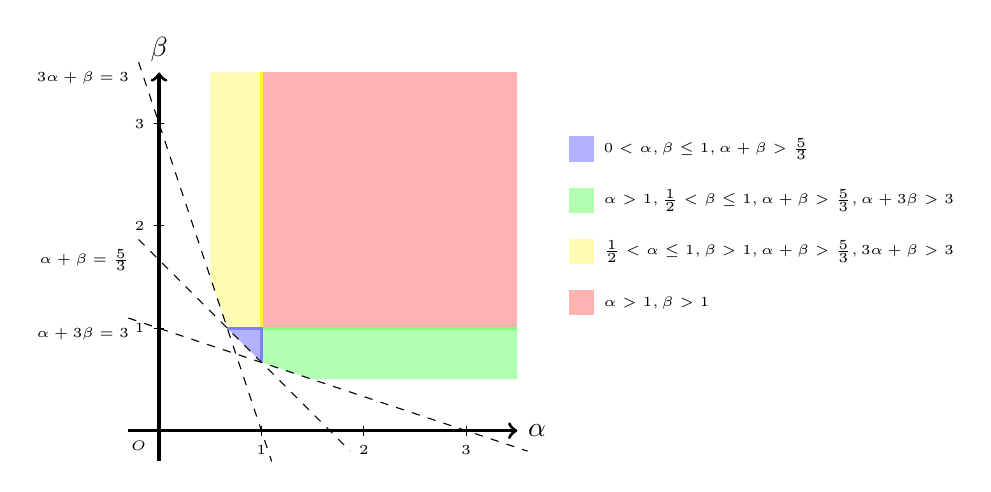
\begin{tikzpicture}[scale=1.3]
       % axes
       \draw[very thick,->] (-0.3,0) -- (3.5,0) node[right] {$\alpha$};
       \draw[very thick,->] (0,-0.3) -- (0,3.5) node[above] {$\beta$};
       % regions and boundaries
       \foreach \x in {1,...,3} \draw (\x, 0.05) -- (\x, -0.05) node[below] {\tiny \x};
       \foreach \y in {1,...,3} \draw (-0.05, \y) node[left] {\tiny \y} -- (0.05, \y);
       \fill[red!30] (1,1) -- (1,3.5) -- (3.5,3.5) -- (3.5,1) --cycle;
       \fill[yellow!30] (1/2,3/2) -- (2/3,1) -- (1,1) -- (1,3.5) --(1/2,3.5)--cycle;
       \fill[green!30] (3/2,1/2) -- (1,2/3) -- (1,1) -- (3.5,1) --(3.5,1/2)--cycle;
       \fill[blue!30] (2/3,1) -- (1, 2/3) -- (1,1) --cycle;
       \draw (-0.2,-0.01) node[below] {\tiny $O$};
       \draw[yellow!80, very thick] (1,1) -- (1,3.5);
       \draw[green!50, very thick] (1,1) -- (3.5,1);
       \draw[blue!50, very thick] (2/3,1)--(1,1)--(1,2/3);
       % labels
       \fill[blue!30] (4,3.25-0.625)--(4.25,3.25-0.625)--(4.25,3.5-0.625)--(4,3.5-0.625);
       \draw (4.25,3.375-0.625) node[right] {\tiny$0<\alpha,\beta\le 1,\alpha+\beta>\frac{5}{3}$};
       \fill[yellow!30] (4,2.25-0.625) -- (4.25,2.25-0.625) -- (4.25, 2.5-0.625) -- (4,2.5-0.625);
       \draw (4.25, 2.375-0.625) node[right] {\tiny$\frac{1}{2}<\alpha\le 1,\beta>1,\alpha+\beta>\frac{5}{3},3\alpha+\beta>3$};
       \fill[green!30] (4,2.75-0.625) -- (4.25, 2.75-0.625) -- (4.25,3-0.625)--(4,3-0.625);
       \draw (4.25,2.875-0.625) node[right] {\tiny$\alpha>1,\frac{1}{2}<\beta\le 1,\alpha+\beta>\frac{5}{3},\alpha+3\beta>3$};
       \fill[red!30] (4,1.75-0.625) -- (4.25, 1.75-0.625) -- (4.25,2-0.625) -- (4,2-0.625);
       \draw (4.25,1.875-0.625) node[right] {\tiny $\alpha>1,\beta>1$};
       % lines and equations
       \draw[dashed] (-1/5,18/5)node[below left]{\tiny $3\alpha+\beta=3$} --(1.1,-0.3);
       \draw[dashed] (-0.3,1.1)  --(18/5,-1/5);
       \draw (-1/5,1.1) node[below left]{\tiny $\alpha+3\beta=3$};
       \draw[dashed] (-1/5,28/15) node[below left]{\tiny $\alpha+\beta=\frac{5}{3}$}-- (28/15,-1/5);
    \end{tikzpicture}
    \caption{The range of $(\alpha,\beta)$ ensures $\int _{\R^2}K^2\,\d x \mathrm{d}y$.}
    \label{fig1}
    \end{figure}

%\begin{figure}[ht]
%    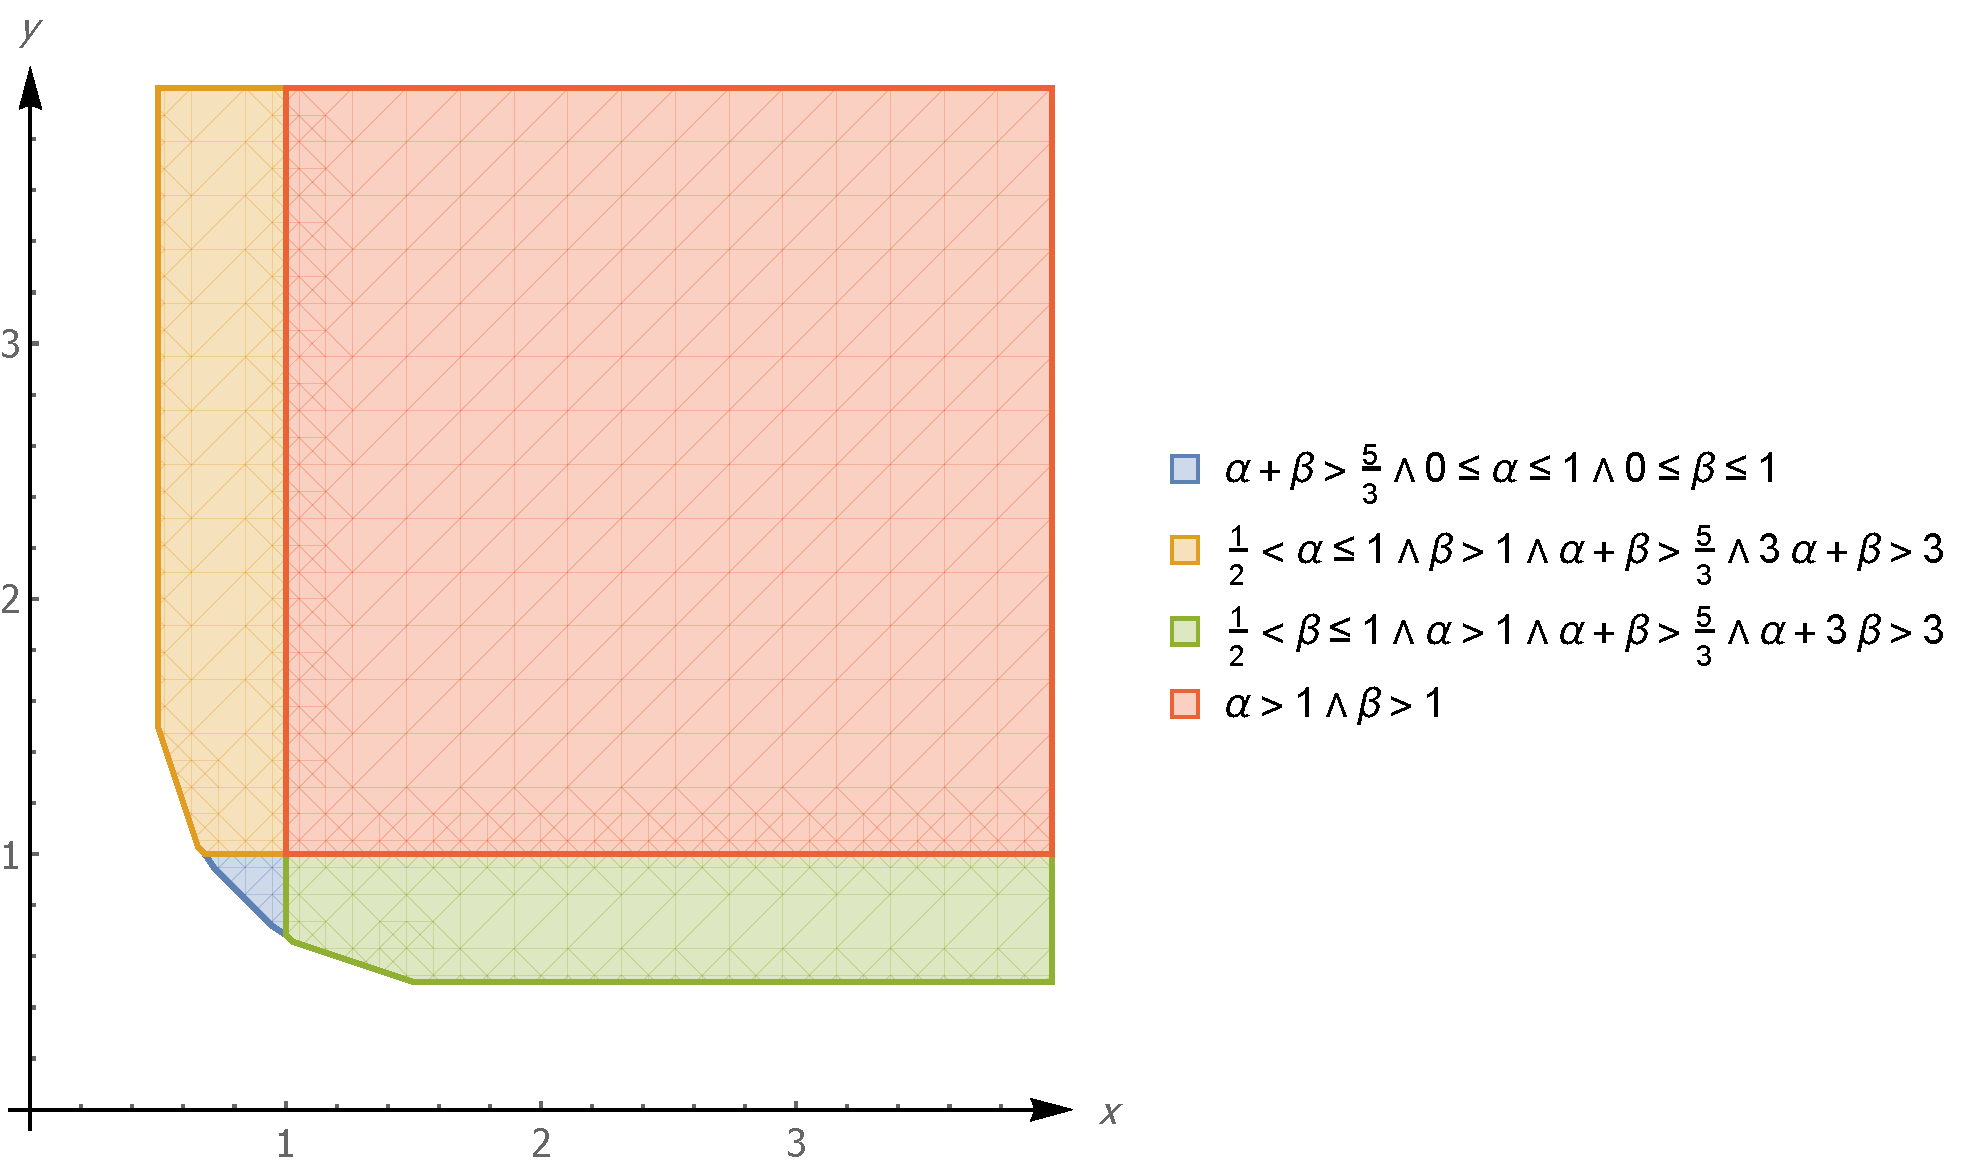
\includegraphics[width=14cm]{range.pdf}
%    \centering
%    \caption{The range of $(\alpha,\beta)$  ensures $\int_{\R^2}K^2\d x \d y<\infty$.}
%    \label{fig1}
%    \end{figure}
 \end{proof}
To obtain Theorem \ref{thm-2}, we need the following unique continuation result.
\begin{lemma}\label{lem-ucp}
    Let $u(t,x)\in C(\R, L^2(\R))$ be a  solution of $\partial_tu+\partial_x^3u=0$. If there exist two time points $t_1\neq t_2$ such that
    \begin{equation}
        \mathrm{supp }\, u(t_j,\cdot)\subset (-\infty,c),\quad j=1,2
    \end{equation}
    or
    \begin{equation}
        \mathrm{supp }\, u(t_j,\cdot)\subset (c,\infty),\quad j=1,2
    \end{equation}
    for some $c\in \R$, then
    $$
        u(t,x)\equiv 0,\quad -\infty <t,x<\infty.
    $$
\end{lemma}
\begin{proof}
See Theorem 3.1 in \cite[p.~60]{zhang-kdv}.
\end{proof}

\begin{proof}[\bf \textit{Proof of Theorem \ref{thm-2}}.] Fix $t>0$. Similar to the proof of Theorem \ref{thm-2}, it suffices to show that $$
\|T\|_{L^2(\R)\to L^2(\R)}\neq 1.
$$
We argue by contradiction. Suppose that $\|T\|_{L^2(\R)\to L^2(\R)}= 1$. Thanks to Lemma \ref{lem-comp-2}, we know $T$ is a compact operator from $L^2(\R)$ to $L^2(\R)$. Thus, there exists $f\in L^2(\R)$ so that
\begin{align}\label{equ-51-5}
\|Tf\|_{L^2(\R)}=\|\chi_BS(t)\chi_Af\|_{L^2(\R)}=\|f\|_{L^2(\R)}=1.
\end{align}
With \eqref{equ-51-5} in hand, it follows from Lemma \ref{lem-2} that $\mathrm{supp }\, f\subset A$ and $\mathrm{supp }\, S(t)f \subset B$. Let $u(\tau,\cdot)=S(\tau)f$. Then $u(\tau,\cdot)$ is a solution of the equation
$$
\partial_\tau u+\partial_x^3u=0.
$$
By the assumption on $A,B$, we have either $\mathrm{supp }\,u(\tau,\cdot)\subset (-\infty,c)$ or $(c,\infty)$ for $\tau=0,t$, according to Lemma \ref{lem-ucp}, we conclude that $u(\tau,\cdot)\equiv 0$. In particular, this implies that $f=0$. But this is impossible since $\|f\|_{L^2(\R)}=1$ by \eqref{equ-51-5}. So we complete the proof. \end{proof}
%
%\section{Generalization}
%\begin{definition}
%    Let $S$ be a linear operator mapping the Hilbert space $(\mathcal{H}(R^n),\|\cdot\|)$ into itself and $E\subset \R^n$ be a measurable set. We call the operator $S$ antilocal with respect to $O$  if for any $f\in\mathcal{H}$
%    $$
%        \chi_Of=\chi_O Sf=0\Rightarrow f=0.
%    $$
%    If the above is true for any measurable set $|O|>0$, then we call the operator $S$ completely antilocal.
%\end{definition}
%We can abstract and generalize the proof of Theorem \ref{thm-2} to the following theorem directly.
%\begin{theorem}\label{thm-4}
%    Let $(\mathcal{H}(\R^n),\|\cdot\|)$ be an infinite-dimensional complex Hilbert space. Let $A$ and $B$ be two measurable sets. Define $Ef=\chi_B f$ and $Ff=\chi_A f$. $S:\mathcal{H}\to \mathcal{H}$ is an invertible linear operator which satisfies $\|S^{-1}\| \|T\|<1$. If $S$ is antilocal with respect to some measurable set $O$ and $A,B\subset O $, then the inequalities (\ref{gen-1}) and (\ref{gen-2}) in Theorem \ref{thm-3} still holds.
%\end{theorem}
%\begin{example}
%    The Hilbert transform
%    $$
%        Hf(x)\equiv \mathrm{p.v.}\frac{1}{\pi}\int_{\R}\frac{f(x-t)}{t}\d t
%    $$
%      is completely antilocal\cite[p.~485]{HavJor} and an isometry in $L^2(\R)$. Then we can use Theorem \ref{thm-4} to obtain the following: Let $A$ and $B$ be two measurable sets with finite measure, then there exists a constant $C=C(n,A,B)$
%    $$
%        \int_{\R}|f|^2\d x\le C\left(\int_{A^c} |f|^2\d x+\int_{B^c}|Hf|^2\d x\right).
%    $$
%
%\end{example}

\section*{Acknowledgements}

This work is partially supported by the National Natural Science Foundation of China under grant No.11701535, and the Fundamental Research Funds for the Central Universities, China University of Geosciences(Wuhan) under grant No.CUGSX01.

\begin{thebibliography}{999}

{\scriptsize


\bibitem{Amrein} W. O. Amerin, A. M. Berthier, On support properties of $L^p$-functions and their Fourier transforms, J. Funct. Anal. 24 (1977) 258--267.


\bibitem{EKPV-kdv}  L. Escauriaza, C. E. Kenig, G. Ponce, L. Vega, On uniqueness properties of solutions
of the k-generalized KdV equations, J. Funct. Anal.  244 (2007) 504--535.

\bibitem{EKPV12}  L. Escauriaza, C. E. Kenig, G. Ponce, L. Vega, Uniqueness properties of solutions to Schr\"{o}dinger equations,
Bull. Amer. Math. Soc. (N.S.) 49 (2012) 415--442.

\bibitem{Havin} V. Havin, B. J\"{o}ricke,  The Uncertainty Principle in Harmonic Analysis, Springer-Verlag, 1994.


\bibitem{Huang} S. Huang, A. Soffer, Uncertainty principle, minimal escape velocities and observability
inequalities for Schr\"{o}dinger equations,  preprint (2017) arXiv:1709.09485,   to appear in Amer. J. Math.

\bibitem{HWW} S. Huang, G. Wang, M. Wang, Observable sets, potentials and Schr\"{o}dinger equations, preprint (2020) arXiv:2003.11263.

\bibitem{Jaming} P. Jaming, Nazarov's uncertainty principles in higher dimension, J. Approx. Theory 149 (1)(2007) 30--41.

\bibitem{LW} Z. Li, M. Wang, Observability inequality at two time points for KdV equations, SIAM J. Math. Anal. 53(2)(2021) 1944--1957.

\bibitem{L-Ponce14} F. Linares, G. Ponce, Introduction to nonlinear dispersive equations, 2nd edition. Springer, 2014.


\bibitem{Nazarov} F. L. Nazarov, Local estimates for exponential polynomials and their applications to inequalities of the
uncertainty principle type, Algebra i analiz 5(4)(1993) 3--66.

\bibitem{Rosier} L. Rosier, B. Y. Zhang,  Exact boundary controllability of the nonlinear Schrodinger equation, J. Differential Equations 246(2009) 4129--4153.

\bibitem{stein} E. M. Stein, R. Shakarchi, Complex analysis, Princeton Lectures in Analysis, 2. Princeton University Press, Princeton, NJ, 2003.

 \bibitem{WWZ}  G. Wang, M. Wang, Y. Zhang, Observability and unique continuation inequalities for the Schr\"{o}dinger equation, J. Eur. Math. Soc.  21 (2019) 3513--3572.


\bibitem{wang21} M. Wang, Z. Li, S. Huang, Unique continuation inequalities for nonlinear Schr\"{o}dinger equations based on uncertainty principles, to appear in Indiana Univ. Math. J.

\bibitem{Yosida} K. Yosida, Functional Analysis, Classics Math., the sixth 1980 edition, Springer-Verlag, Berlin, 1999.


\bibitem{zhang-kdv} B. Y. Zhang,   Unique continuation for the Korteweg-de Vries equation, SIAM J. Math. Anal. 32 (1992)  55--71.

\bibitem{zhang-sch} B. Y. Zhang,   Unique continuation for the nonlinear Schr\"odinger equation, Proc. Roy. Soc. Edinburgh Sect. A 127 (1997)  191--205.
     }
\end{thebibliography}

\end{document}
